\documentclass[a4paper,fleqn,usenatbib,useAMS]{mnras}

%\usepackage[draft]{graphicx}  % this stop figures from rendering
\usepackage{graphicx}	% Including figure files
\usepackage{amsmath}	% Advanced maths commands
\usepackage{amssymb}	% Extra maths symbols
\usepackage{multicol}        % Multi-column entries in tables
\usepackage{bm}		% Bold maths symbols, including upright Greek
\usepackage{pdflscape}	% Landscape pages
\usepackage{IEEEtrantools} % for stacked equations

\newcommand{\numax}{\ensuremath{\nu_{\textrm{max}}}}
\newcommand{\dnu}{\ensuremath{\Delta\nu}}
\newcommand{\teff}{\ensuremath{T_{\textrm{eff}}\:}} 
\newcommand{\kep}{\ensuremath{Kepler}\:}
\newcommand{\pdet}{\ensuremath{P_{\rm det}\:}}
\newcommand{\kp}{\ensuremath{K_{p}\:}}
\newcommand{\tobs}{\ensuremath{T_{\textrm{obs}}\:}} 
\newcommand{\imag}{\ensuremath{I_{\textrm{mag}}\:}} 

\newcommand{\bibtex}{\textsc{Bib}\!\TeX} % bibtex. Not quite the correct typesetting, but close enough

\usepackage[T1]{fontenc}
\usepackage{ae,aecompl}
%\usepackage{newtxtext,newtxmath}  % new version
\usepackage{txfonts}  % old version

\title[TRG]{TESS Asteroseismic Predictions for Red Giants using Machine Learning}

\author[M. Schofield et al.]{M. Schofield$^{1, 2}$\thanks{E-mail: mxs191@bham.ac.uk}, G. R. Davies$^{1, 2}$, W. J. Chaplin$^{1, 2}$, M. F. Randrianandrasana
\\
% List of institutions
$^{1}$Department of Physics and Astronomy, the University of Birmingham, Birmingham B15 2TT, UK \\
$^{2}$Stellar Astrophysics Centre (SAC), Department of Physics and Astronomy, Aarhus University, Ny Munkegade 120, DK-8000 Aarhus C, Denmark}


%\thanks{Contact e-mail: \href{mailto:mxs191@bham.ac.uk}{mxs191@bham.ac.uk}}\thanks{Present address: Department of Physics and Astronomy, the University of Birmingham, Birmingham B15 2TT, UK}



\date{Last updated 2017 May 31; in original form 2017 May 31}
\pubyear{2018}

\begin{document}
\label{firstpage}
\pagerange{\pageref{firstpage}--\pageref{lastpage}}
\maketitle

\begin{abstract}
{\it Summary}: This paper presents a method to predict Red Giant mode detectability with TESS using a Machine Learning Classifier. It requires only the global parameters \dnu, \numax, [M/H], \teff, the stellar magnitude and length of observation. \newline
{\it Method}: Lightcurves for \kep \ stars with fitted radial mode frequencies were used to generate equivalent TESS lightcurves. The length of observation was reduced, \kep \ white noise was removed, the bandpass was adjusted, and TESS white noise was added. A detection test was then run on 3 observed modes in these 'TESS-like' lightcurves. Classifiers were then used to predict mode detectability with TESS based upon the global asteroseismic and spectroscopic parameters. The Classifier successfully predicted mode detectability in the original \kep stars, and for 1 year of TESS-like data.\newline
{\it Application}: By changing only the length of dataset, instrumental noise level and bandpass of observation, this tool can make solar-like detection predictions for future missions such as K2, PLATO and CoRoT. It can make predictions and select targets much faster than traditional detection tests. It is especially useful in an age where extremely large datasets from MAST and Gaia are available (\citet{eisenstein_sdss-iii:_2011}, \citet{gaia_collaboration_gaia_2016}).
\end{abstract}


\section{Introduction}

Satellites such as $Kepler$ have allowed asteroseismology of solar-like and Red Giant stars to advance rapidly since the last century \citet{chaplin_asteroseismology_2013}. Power spectra can now be resolved to detect individual modes of oscillation in Main Sequence and Red Giant stars (\citet{lund_standing_2017}, \citet{davies_asteroseismology_2016}).

Future space missions such as TESS \citep{ricker_transiting_2014}, K2 \citep{howell_k2_2014}, CoRoT \citep{baglin_corot:_2006} and PLATO \citep{rauer_plato_2014} will add to our understanding of stellar structure and evolution. These missions will provide a large amount of high-precision data. More than ever, the field of stellar astrophysics will require tools to perform big-data analysis \citep{kremer_big_2017}. 

%In order to select asteroseismic targets for these missions, the detectability of solar-like oscillations inside these stars needs to be estimated.

One of the tools than can be used to handle the larger amount of data from future missions is Machine Learning. In this work, Machine Learning was used to create a TESS target selection function using the set of $Kepler$ Red Giant stars from \citet{davies_asteroseismology_2016}. This publicly-available algorithm\footnote{https://github.com/MathewSchofield/TRG} can be downloaded and used as a target selection function for any future space mission.

In most situations Machine Learning is used to solve problems in one of two ways: either by using Supervised or Unsupervised Learning. Supervised Learning involves problems where there is a known result. 

Supervised Learning has been used to classify types of variable star using previously labelled data (\citet{nun_supervised_2014}, \citet{elorrieta_machine_2016}). This previously labelled data is known as training data: this is used to train the Machine Learning algorithm. In the problem of variable stars, lightcurves that had already been classified were used to train the algorithm (this is the training dataset). This algorithm was then used to classify the lightcurves of unidentified stars (this is known as the testing dataset).

In Unsupervised Learning, there are no known results/labels. The aim of Machine Learning in this case would be to find trends between variables. This has been be used to identify similar stars by analysing their lightcurves without using previously labelled data \citep{valenzuela_unsupervised_2018}).

The aim of this work is to use Machine Learning to make predictions about mode detectability (\pdet) in Red Giant stars. In this case, \pdet is a known label, so this is a Supervised Learning problem\footnote{https://machinelearningmastery.com}.

Within Supervised Learning, two common algorithms that are used are Classification and Regression. In Regression, the relationship between variables is interpreted using a measure of uncertainty (such as using $\chi^{2}$ tests). Models are fitted using the independent data, and uncertainty is measured. The models are then improved by reducing this uncertainty. Note that regression is used when the label is continuous. For example, predicting the magnitude of a star is a problem suited to regression, as a star can have any magnitude \citep{steinhardt_nonparametric_2018}.

Conversely, Classification algorithms work by assessing similarity\footnote{http://www.simafore.com}. In Classification, the training set is separated into groups based on the similarity of the data. The more information that was gained by splitting the data, the better. For example, if the problem were to separate Red Giant stars from Main-Sequence stars, a star could be classified as either a Red Giant (1), or not a Red Giant (0). In this example, having a Luminosity above $\sim10L_{\odot}$ would be a strong indicator that the star was a Red Giant so the data could be separated into groups here. The Classifier would continue to separate the dataset until the Red Giant and Main Sequence samples were distinct. This is not the only problem where Classification can be used on Red Giant stars (\citet{ness_cannon_2015}, \citet{wu_mass_2017}).

In this work, individual fitted modes from \citet{davies_asteroseismology_2016} were used to make asteroseismic predictions for TESS with a Supervised Classifier. By separating the targets into those with detected modes and those without, a Classifier was used to select the optimal targets for future observation.

Firstly, Section \ref{sect: size} describes how the size of the datasets were increased to improve the predictive ability of the Classifier. Section \ref{sect: dataset} then describes how the timeseries of every star were treated before transforming them into power spectra. Section \ref{sect: det_test} goes on to describe the detection test that was run on the solar-like oscillations. This returned a probability of detection \pdet for every mode. Each mode was grouped into a discrete class depending upon it's detection probability; each mode was either very likely to be observed (2), quite likely (1), or unlikely (0).

Lastly, Section \ref{sect: classifier} describes the classification of stars into a group with detected modes, and a group without. This was done by giving a Supervised Classifier asteroseismic and spectroscopic information on every target from APOKASC \citep{pinsonneault_apokasc_2014}. 70\% of the stars were used to train the Classifier; 30\% of the sample was kept to test the algorithm. The Classifier was given global asteroseismic and spectroscopic information, as well as mode detection probabilities of the stars in the training set. It then made predictions about mode detectability on the testing set.

The Classifier recognised patterns between the variables in the training set, and successfully made predictions about mode detectability with a 0.98\% precision for the original \kep data. It achieved a precision of 0.92 for 1 year of TESS-like observation, and 0.74 for 27 days of TESS-like observation.



\section{Increasing the size of the datasets}
\label{sect: size}

Machine Learning performs best when a large dataset is available to train the algorithm on. In order to increase the size of the dataset from \citet{davies_asteroseismology_2016} above 1000, the magnitude of each \kep star was perturbed. Each star had it's magnitude perturbed 100 times before the lightcurves were transformed to TESS-like power spectra. 

The noise functions of \kep and TESS were used as PDFs to draw magnitudes from. These were used because they provide realistic distributions of the number of stars at different magnitudes that the satellites observed/will observe. Many more fainter stars are observed than brighter stars because the volume of space that contains stars increases as the distance of observation increases.

The noise function of \kep depends on the \kep magnitude of the star, $K_{p}$. This noise function is from \citet{chaplin_predicting_2011}. It is given by
\begin{equation}
\sigma = \frac{10^{6}}{c} \times \sqrt{c+9.5 \times 10^{5}\Bigg(\frac{14}{K_{p}}\Bigg)^{5}} ,
\label{eq:kep noise}
\end{equation}
where
\begin{equation}
c = 1.28 \times 10^{0.4(12-K_{p})+7} .
\end{equation}

Similarly, the noise function of TESS was estimated using the `calc noise' IDL procedure (from William Chaplin, private communication), which depends on the $I_{c}-$band magnitude of the star and the number of pixels in the photometric aperture used when observing the star. This is given by
\begin{equation}
N_{\rm aper} = 10 \times (n+10) , 
\end{equation}
where $n$ is
\begin{equation}
\label{eq:tess noise}
n = 10^{-5.0} \times 10^{ 0.4 \times (20-I_{\rm mag})} .
\end{equation}

These noise functions were used as the PDFs to draw stellar magnitudes from. 100 magnitudes were drawn for every \kep Red Giant. After removing gaps in the data, this left 60,000 samples. The lightcurves of this much larger \kep dataset were then degraded to look like TESS observations.


\section{Transforming the lightcurves}
\label{sect: dataset}

Before a Classifier could be used on the large Red Giant sample, the timeseries data from \kep needed to be adjusted for a different satellite and mission. This could either be done in the time or frequency domains. Adjustments were made in both domains, and the results were compared. %The time domain method was chosen to transform the lightcurves, and was used in the rest of this work.

Several different adjustments needed to be made to the \kep \ data. One difference between the missions is the length of observation. The \kep \ mission observed for 4 years, while TESS' nominal 2 year mission will observe stars for between 27 days to 1 year, according to the star's ecliptic latitude (Figure \ref{TESS field}). This distinction can be clearly seen when comparing the timeseries', see Figure \ref{ts plot}.

\begin{figure}
	\centering
	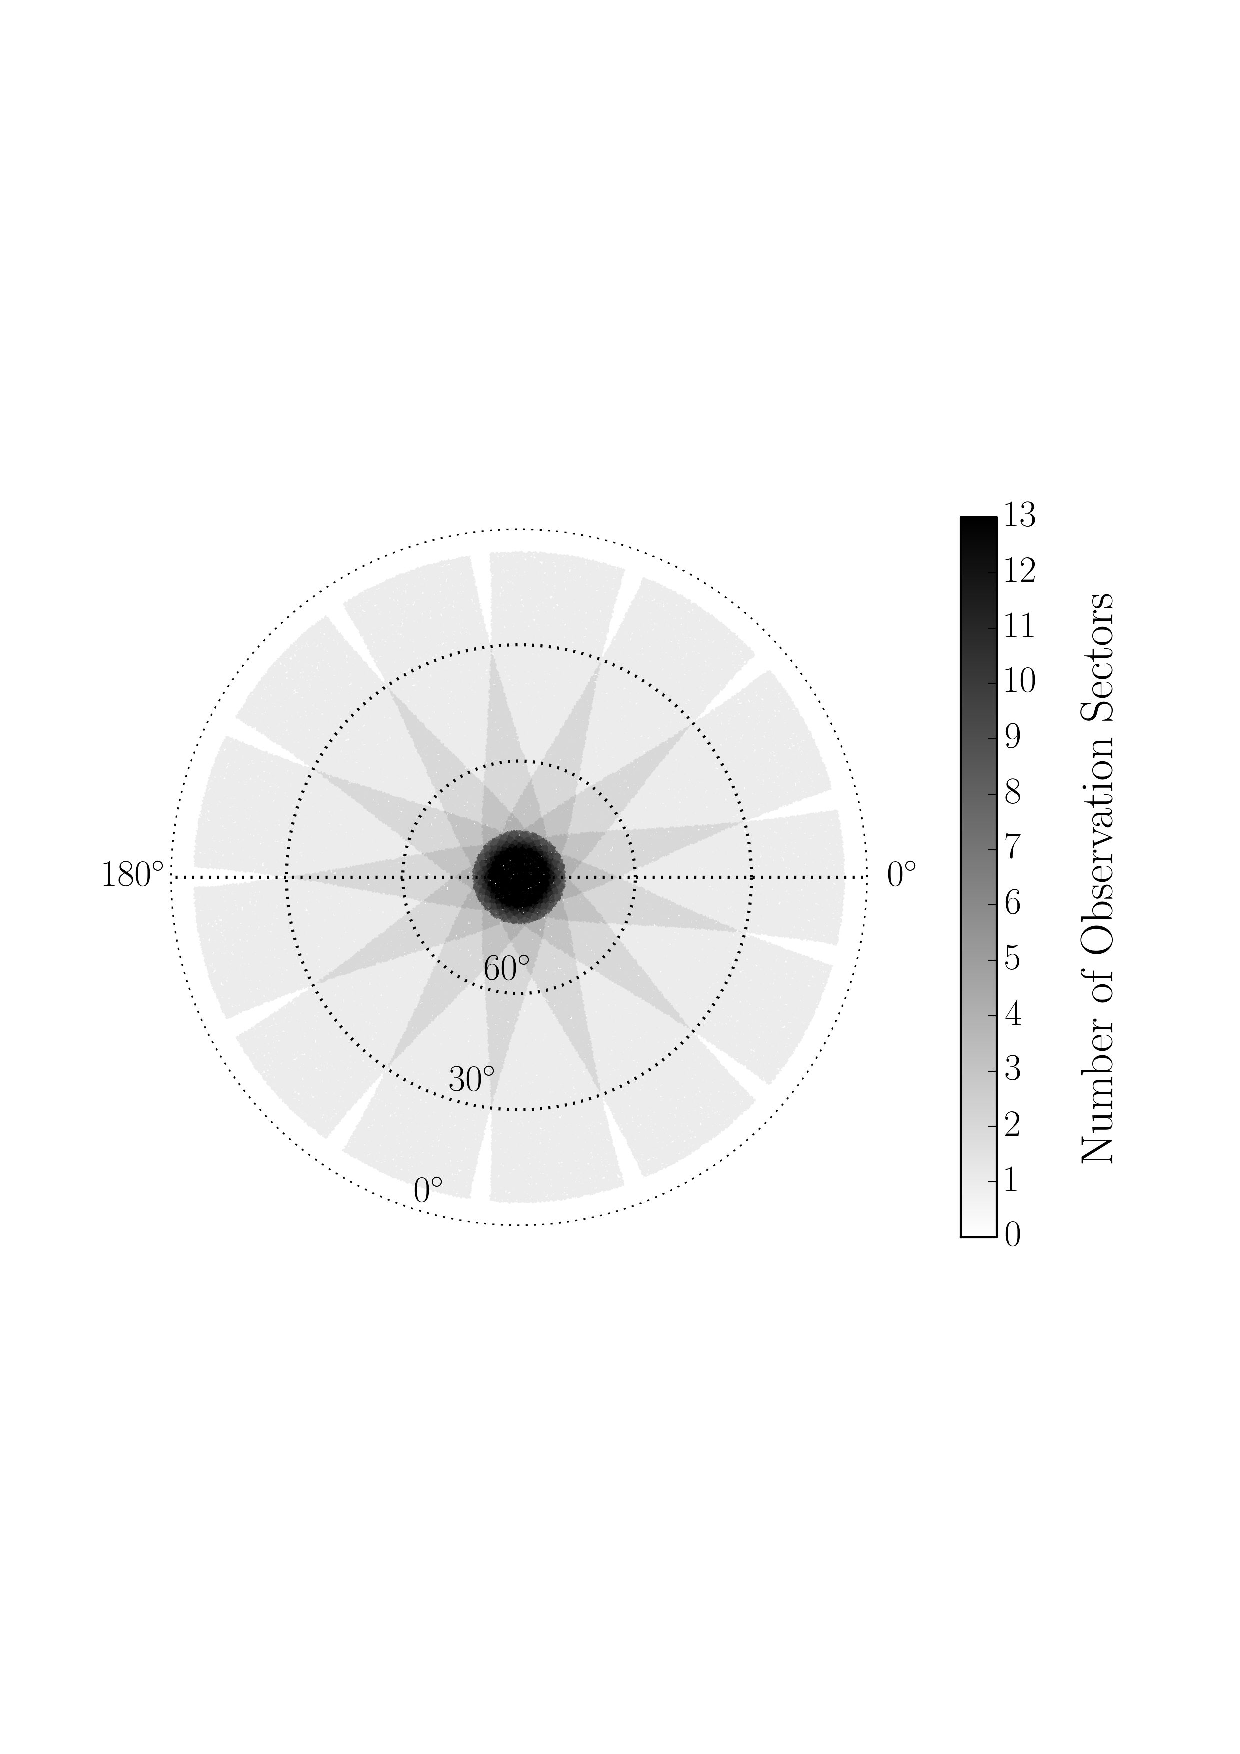
\includegraphics[scale=0.4]{cropped_TESSfield.pdf}
	\caption{TESS field of view, centred around the ecliptic pole. Each strip will be observed for 27 days before the satellite rotates. Image taken from \citet{campante_asteroseismic_2016}.}	
	\label{TESS field}
\end{figure} 

\begin{figure}
	\centering
	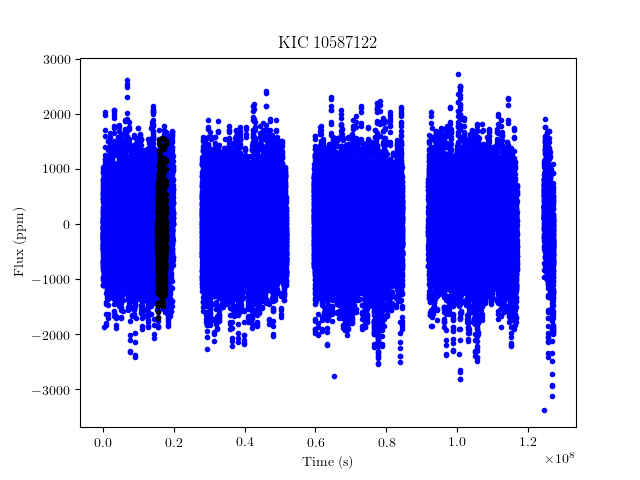
\includegraphics[scale=0.6]{timeseries_10587122}
	\caption{The 4-year long Power Spectra of KIC 10587122 is plotted in blue. Overplotted is the 27-day time segment with most coverage (the period with fewest gaps in the data). Reducing the length of observation this drastically will badly hamper mode detectability.}	
	\label{ts plot}
\end{figure} 

As well as reducing the dataset length, the bandpass of observation needed to be adjusted. TESS will observe in a much redder bandpass than that of \kep, Figure \ref{bandpass}. This has the effect of reducing the amplitude of stellar signals (i.e the signals due to stellar granulation and oscillation), while leaving the white noise component unaltered. \citet{campante_asteroseismic_2016} found this bandpass correction to be 0.85 for TESS.

\begin{figure}
	\centering
	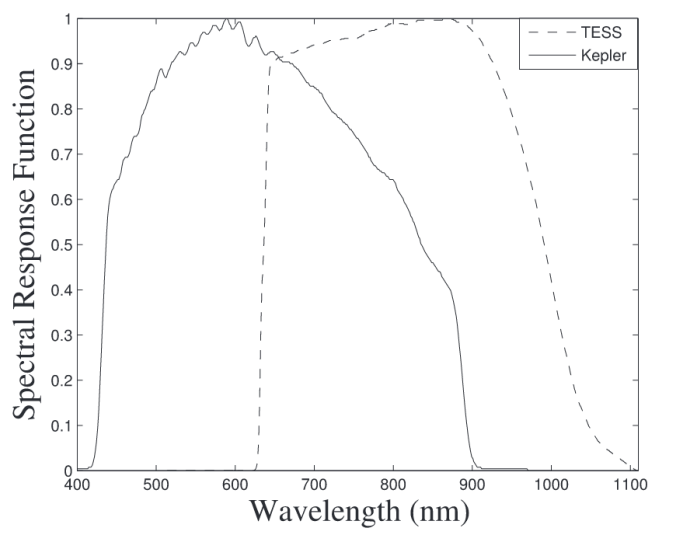
\includegraphics[scale=0.4]{bandpass.png}
	\caption{The bandpass' of the $Kepler$ and TESS missions. TESS will observe at longer (i.e redder) wavelengths than $Kepler$. This will reduce the amplitude of oscillations and granulation, whilst the white noise level will by unaffected. Image taken from \citet{placek_combining_2016}.}	
	\label{bandpass}
\end{figure} 

Thirdly, the instrumental noise level in \kep \ is different to the noise level in TESS. The noise level for the \kep \ satellite depends on the \kep \ magnitude of the star, equation \ref{eq:kep noise}.

Instrumental noise from TESS needed to be added to the timeseries'. This noise level was estimated using equation \ref{eq:tess noise}, along with the `calc noise' IDL procedure (from William Chaplin, private communication).

These three adjustments - the length of observation, the bandpass, and the noise level - were performed in both the time and frequency domains for comparison. The methods used are described in Figures \ref{ts flowchart} and \ref{fr flowchart}. The resulting Power Spectra are compared in Figures \ref{Power Spectra} and \ref{overplotted PS}. After comparing the results, the decision was made to perform adjustments in the time domain before transforming to the frequency domain because the background noise level is lower when the time domain method is used to transform the lightcurves to TESS-like power spectra. 

After adjustments were made in the time domain, power spectra were generated for every star. Power spectra were generated for the original 4-year \kep sample, 1 year of TESS observations and 27 days of TESS observations. A detection test was then run on the radial modes of every star in these 3 datasets. 

\begin{figure}
	\centering
	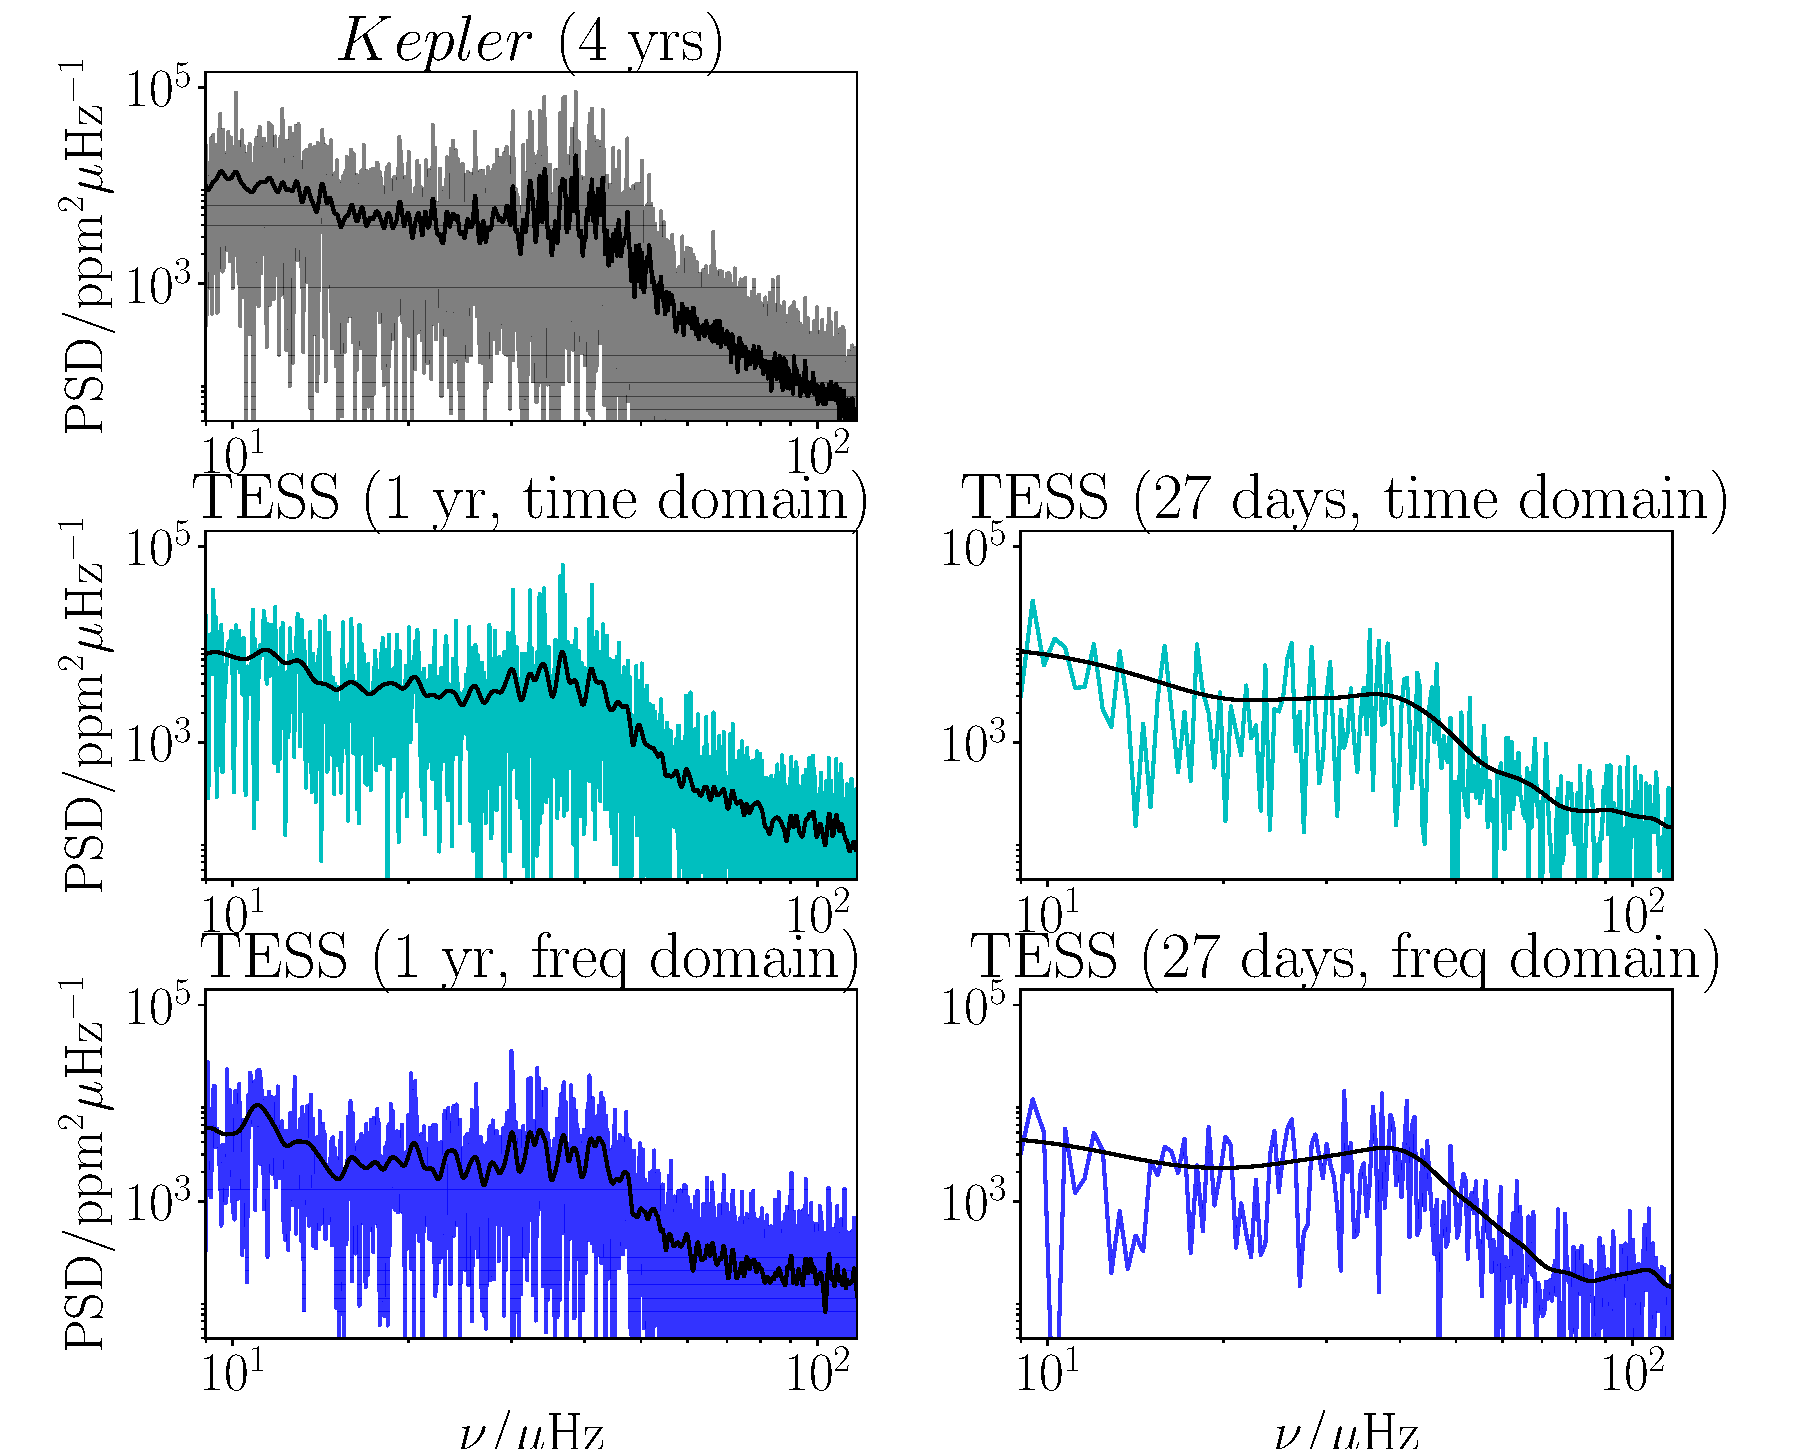
\includegraphics[scale=0.3]{diagnostic_plot1_modes}
	\caption{The Power spectra of KIC 10587122 is plotted five times with moving medians in black. The original Power Spectra is plotted in grey. The power spectra after making the data look like TESS are plotted in blue. The data was transformed in the time domain (light blue) or frequency domain (dark blue). The left column shows 1 year of TESS observation (the maximum). The right column shows 27-days (the minimum). Based on this, the time domain was chosen to transform the data in as the background noise level appears lower.}	
	\label{Power Spectra}
\end{figure} 
\begin{figure}
	\centering
	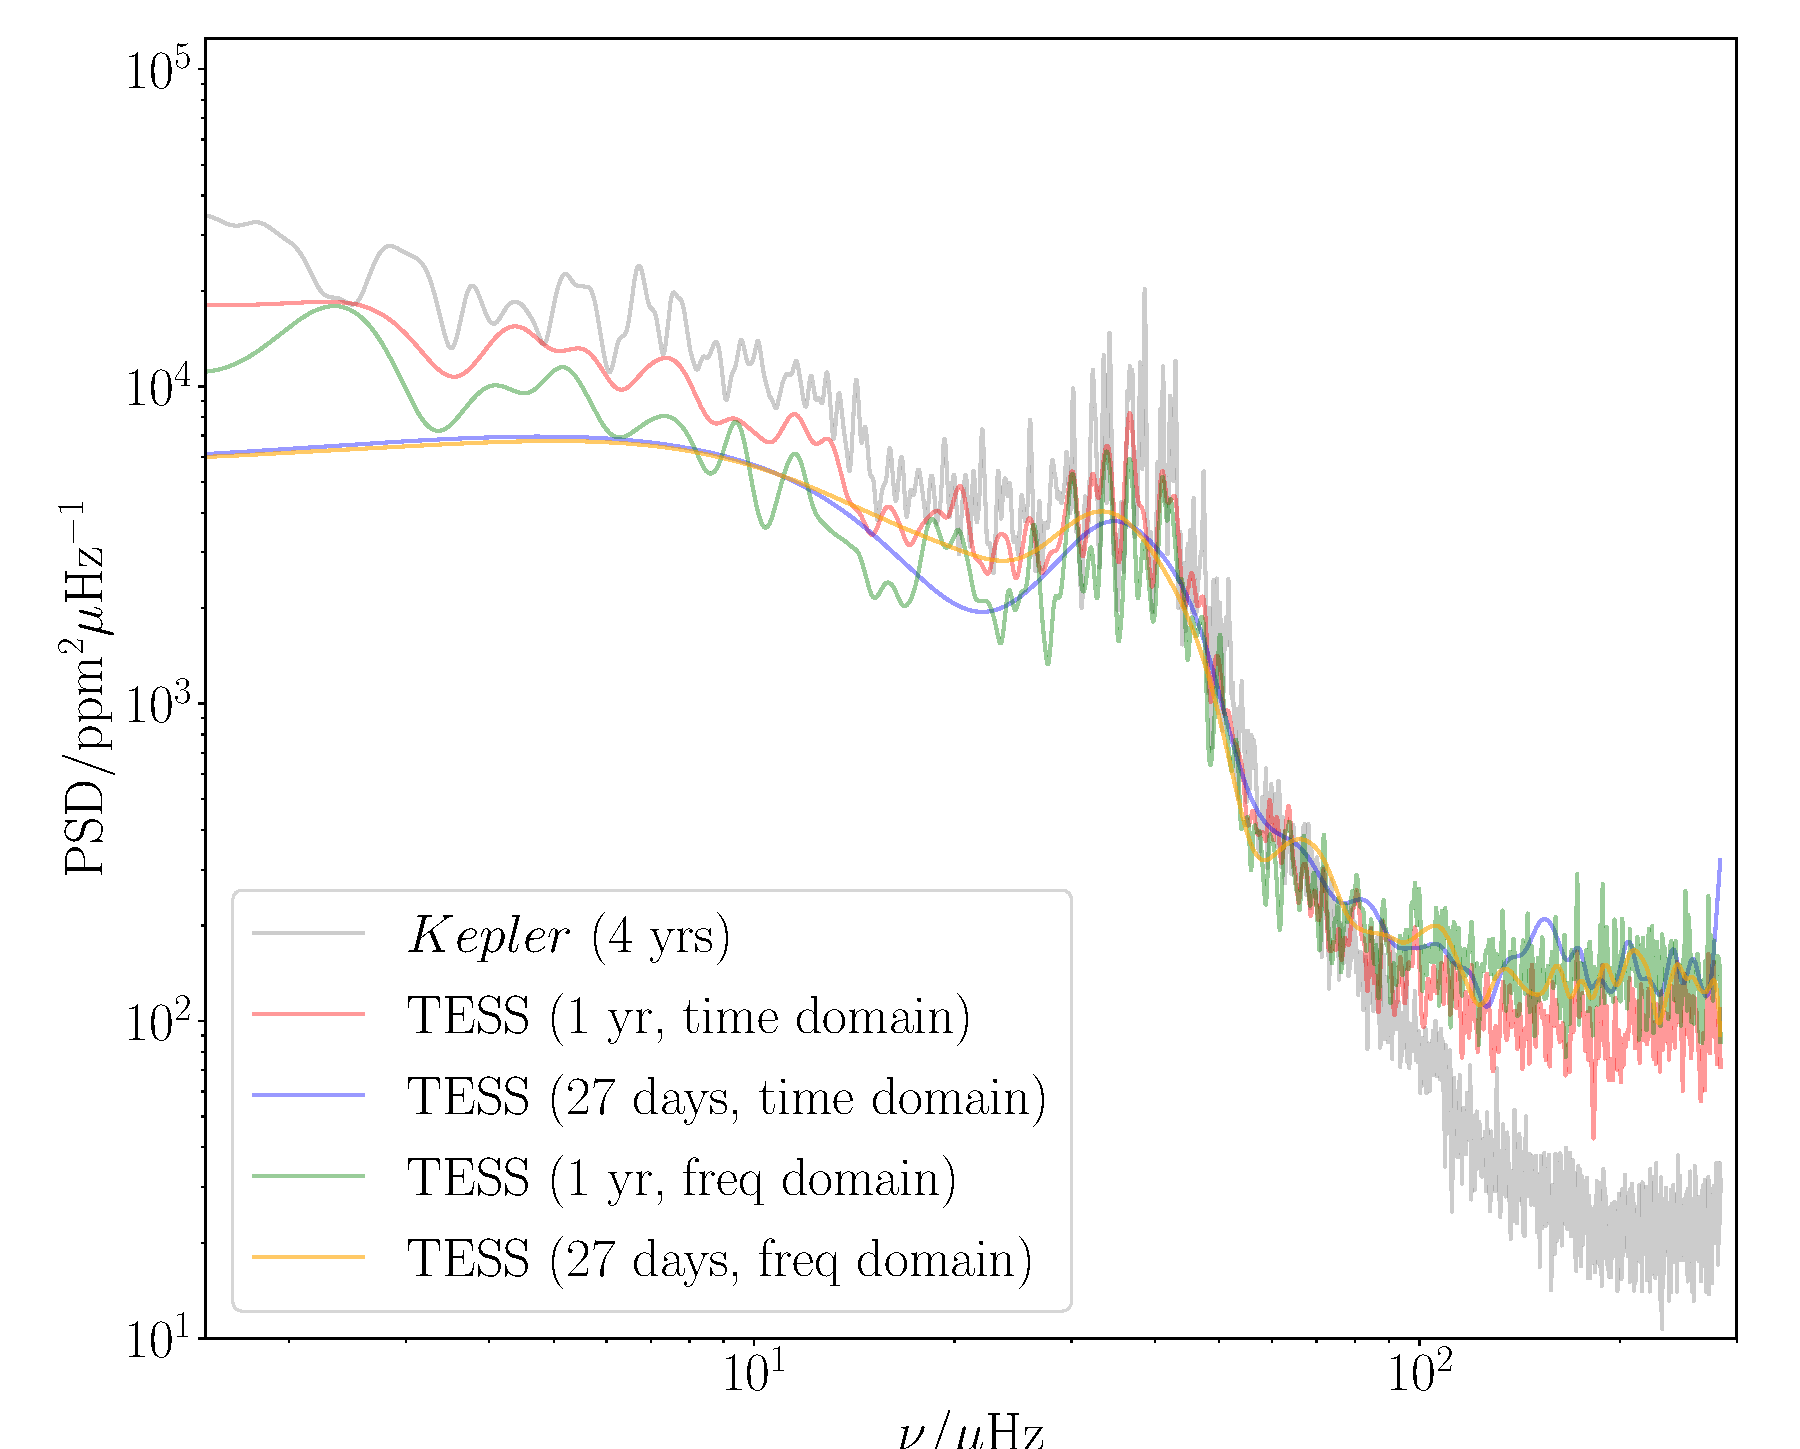
\includegraphics[scale=0.3]{diagnostic_plot2_full}
	\caption{The Power Spectra of KIC 10587122. The original power spectra is in grey. The data was transformed into TESS observation and overplotted. The transformation was done in the time and frequency domains for comparison. Based on this, the time domain was chosen to transform the data in as the background noise level appears lower.}	
	\label{overplotted PS}
\end{figure} 


\onecolumn
\begin{figure}
	\centering
	\includegraphics[scale=0.5, trim={0 3cm 10cm 0}]{"TRG timeseries flowchart".pdf}
	\caption{Flow chart of the method to convert the data from \kep \ to TESS observations in the time domain.}	
	\label{ts flowchart}
\end{figure} 

\begin{figure}
	\centering
	\includegraphics[scale=0.5, trim={0 3cm 0 0}]{"TRG frequency flowchart".pdf}
	\caption{Flow chart of the method to convert the data from \kep \ to TESS observations in the frequency domain.}	
	\label{fr flowchart}
\end{figure}
\newpage
\twocolumn



\section{Detection Test}
\label{sect: det_test}

Section \ref{sect: dataset} described the method to transform the $Kepler$ lightcurves into TESS-like power spectra. A detection test was then run on the stars to determine which modes were visible after observation by TESS, and which were not.

First, a moving median from \citet{davies_asteroseismology_2016} was used to estimate the proportion of the signal that was due to white noise and stellar granulation. The solar-like mode envelope width was used as the frequency range of the moving median. This envelope width was calculated as
\begin{equation}
\Gamma_{\rm env} = 0.66 * \numax^{0.88},
\end{equation}
from \citet{mosser_characterization_2012}. The moving median was used to interpolate between frequencies in the power spectrum. It provided an estimate of the total background in the power spectrum. This background was divided out of the power spectrum to the get Signal-to-Noise ratio of the spectrum,
\begin{equation}
\label{eq:snr}
{\rm SNR} = P/B.
\end{equation}
Once the SNR spectrum for the star was recovered, the SNR values at the mode frequencies were extracted. To ensure the correct SNR values of every mode were used, a window was fitted around each peak-bagged mode frequency. The size of the window was given as the linewidth of the mode. The highest value in the window was taken as the SNR of the mode. An example of this for KIC 7014894 is shown in Figure \ref{snr}.
\begin{figure}
	\centering
	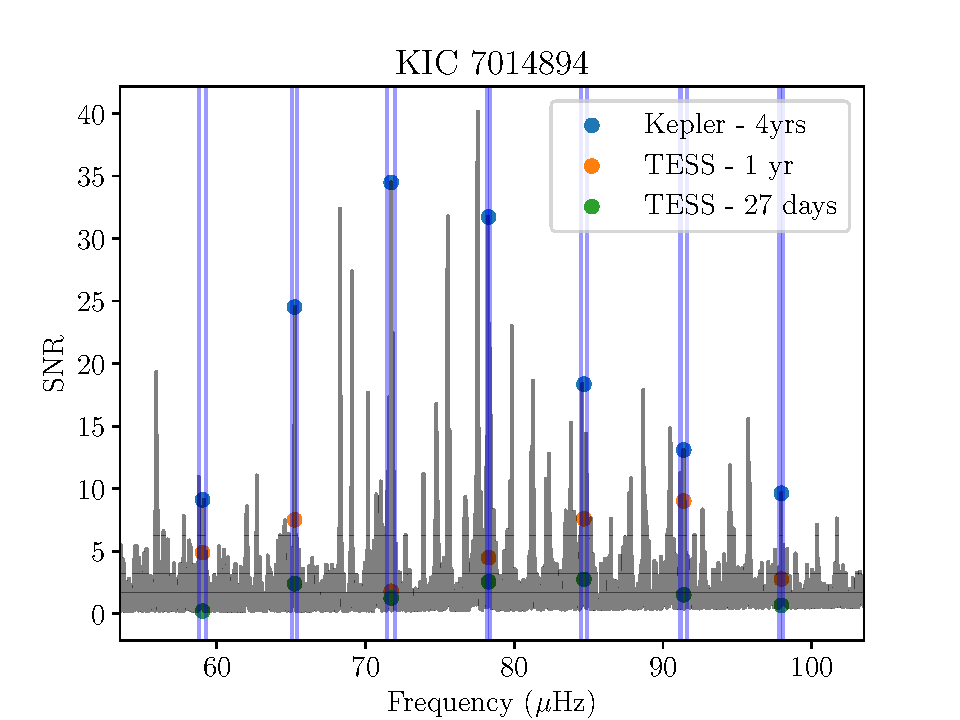
\includegraphics[scale=0.6]{plot4_SNR7014894.pdf}
	\caption{The SNR spectrum of KIC 7014894 after background subtraction. The SNR values of the radial modes in the star were extracted from this spectrum. The values of every mode in the original Kepler spectrum are plotted in blue. The overplotted orange points are the SNR values after degrading the signal to 1 year of TESS observation. Similarly, the green points are the SNR values of 27 days of TESS observations. The white noise level and reduced observation time severely reduce the SNR of TESS observations compared to \kep.}	
	\label{snr}
\end{figure}

Once all mode SNR values for the star were calculated, a detection test was run on each mode \citep{chaplin_predicting_2011}, \citep{campante_asteroseismic_2016}.

The probability $P$ that the SNR of the mode lies above some threshold ${\rm SNR_{thresh}}$ is
\begin{equation}
\label{eq:pdet}
{P \rm ({ SNR \geq SNR_{thresh}})} =  p .
\end{equation}

A false-alarm probability $p$ of 5\% was set; there is a 95\% chance that the signal is due to solar-like oscillations, rather than noise. Equation \ref{eq:pdet} is solved for $\rm SNR_{thresh}$ by substituting $P$ with
\begin{equation}
\label{eq:prob}
P = \int_{x}^{\infty} \frac{e^{-x}}{\Gamma(N)} x^{N-1} dx .
\end{equation}
$\Gamma(N)$ is the Gamma function. The lower bound of Equation \ref{eq:prob} is set to $x=1+{\rm SNR_{thresh}}$. N is the number of frequency bins that the mode occupies. The noise in these bins is assumed to follow $\chi_{2}$ $2n_{\rm bins}$ d.o.f statistics. 

Once $\rm SNR_{thresh}$ is found, Equation \ref{eq:prob} is solved again. This time it is solved for $P$ by setting $x=(1+{\rm SNR_{thresh}})/(1+{\rm SNR})$. Here, SNR is the observed Signal-to-noise Ratio calculated from Equation \ref{eq:snr}. This calculates the probability that the frequency spike was due to stochastic excitation in the convective envelope of the star.

\begin{figure}
	\centering
	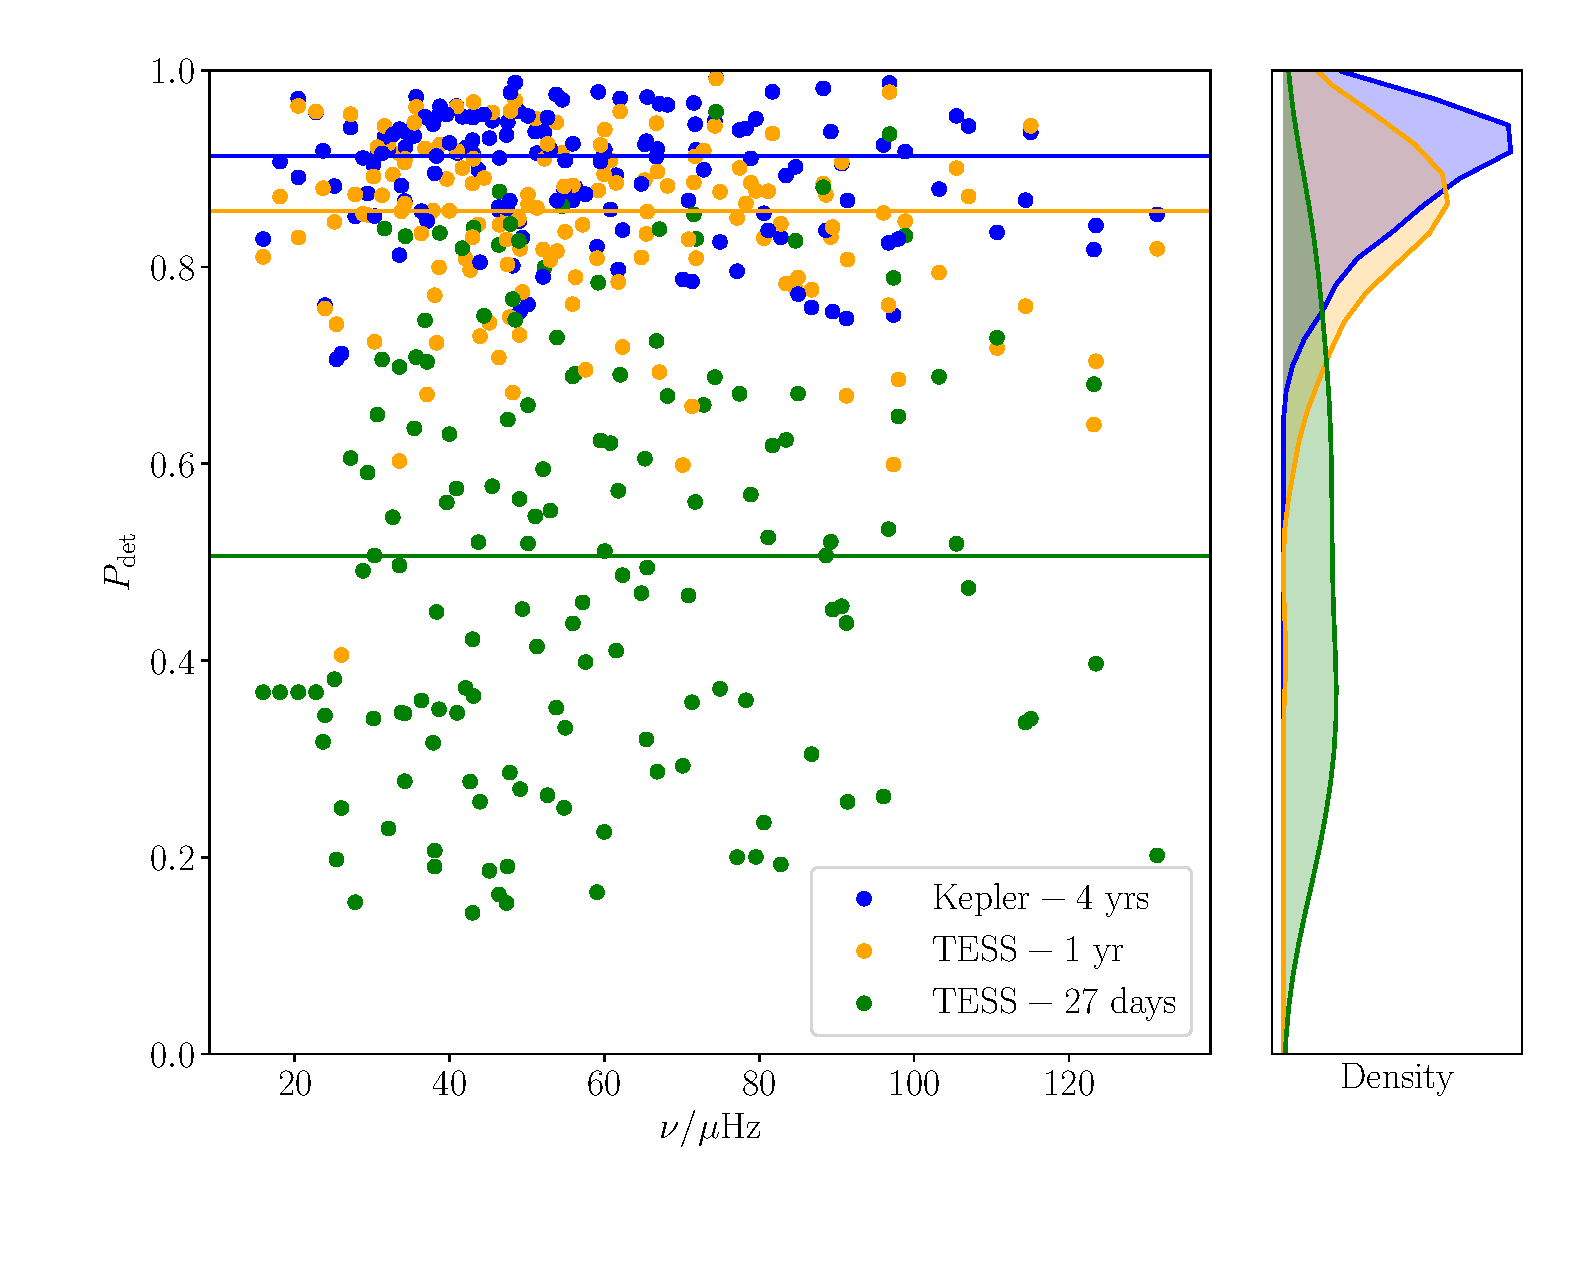
\includegraphics[scale=0.3]{DetTest_Diagnostic_plot3.pdf}
	\caption{A plot showing the result of the detection test, after running on every mode in 20 stars. The results of the original power spectra are plotted in blue. The results of 1 year of TESS observation are in orange. 27 days of TESS observation is in green. At this short an observation, detecting individual modes will be extremely difficult.}	
	\label{fig: modes}
\end{figure}

This detection test was applied to every mode of every star in the sample. Figure \ref{fig: modes} shows the mode detection probabilities from this test for the original \kep dataset, for 1-year of TESS observation and for 27 days of TESS observation. After the \pdet values for the 3 datasets were calculated, a Classifier was used to determine if these results could be predicted rather than calculated. This is described in Section \ref{sect: classifier}.


\section{Classification}
\label{sect: classifier}

Section \ref{sect: dataset} describes how the lightcurves of every star were treated before a detection test was run on the oscillations in Section \ref{sect: det_test}. After this, Classification was applied to the stars to separate them into a suitable target list, and a list of stars that are not suitable for observation with TESS.

It is worth noting that this could be done without using Machine Learning, although it takes much longer. In the age where datasets from missions such as MAST and Gaia \citep{gaia_collaboration_gaia_2016} exist, tools need to be developed to make use of the huge amount of information we now have on stars across the Milky Way. If Machine Learning can replicate the results from a detection test, it could be used as a much faster target selection tool before future observations. It would reduce the computation time needed to generate a list of targets down by orders of magnitude.


\subsection{Preparing the data}
Firstly, the detection probabilities of every mode were taken from Section \ref{sect: det_test}. Each probability was put into a discrete bin (or {\it class}) depending on how likely the mode is to be detected. These discrete classes are given in equation \ref{eq:class}.
\begin{equation}
\label{eq:class}
P_{\rm det} = \left\{ \,
    \begin{IEEEeqnarraybox}[][c]{l?s}
      \IEEEstrut
      2 & if 1.0 $\geq$ \pdet $>$ 0.9  \, , \\
      1 & if 0.9 $\geq$ \pdet $>$ 0.5  \, , \\
      0 & if 0.5 $\geq$ \pdet $>$ 0.0  \, .
      \IEEEstrut
    \end{IEEEeqnarraybox}
\right.
\end{equation}

Using equation \ref{eq:class}, every mode was assigned a discrete class {\texttt [0, 1 or 2]}, depending on how high the probability of detection was for that mode. The same three radial modes ({\it 3 labels}) were used for every star: the mode closest to the centre of the power-excess due to solar-like oscillations $\nu_{\rm max; n}$, the radial mode one overtone below that $\nu_{\rm n-1}$, and one overtone above that, $\nu_{\rm n+1}$ [\pdet(1), \pdet(2), \pdet(3)]. It was important to use the same information for every star so that the algorithm could be trained on the patterns between the variables.

A classifier is an algorithm that can learn a relationship between variables. The classifier will map from some initial information about the star (the X data), to some unknown information (the Y data). In this work, the X data were magnitude ($K_{p}$ or $I_{\rm mag}$), \numax, \dnu, \teff and [Fe/H]. The Y data labels were the \pdet values of 3 radial modes, centred around \numax. An example of the final dataset for 1 year of TESS-like observations are shown in Tables \ref{tab: x dataset} and \ref{tab: y dataset}.





\begin{table}
\begin{center}
\begin{tabular}{|*{7}{c|}}
KIC     & Iteration & \numax & \dnu & \teff & [M/H] & \imag \\
\hline
9205705	& 1         & 25.23	& 3.181 & 4685 & -0.39 & 9.89  \\
9205705	& 2         & 25.23	& 3.181 & 4685 & -0.39 & 9.19  \\
9205705	& 3         & 25.23	& 3.181 & 4685 & -0.39 & 9.79  \\
9205705	& 4         & 25.23	& 3.181 & 4685 & -0.39 & 11.30 \\
...                                                        \\
9205705	& 100       & 25.23	& 3.181 & 4685 & -0.39 & 7.81  \\
2554924	& 1	        & 33.97	& 3.967 	& 4594 &  0.27 & 8.46  \\
2554924	& 2         & 33.97	& 3.967 	& 4594 &  0.27 & 9.26  \\
...                                                         \\
\hline
\end{tabular}
\end{center}
\caption{An example of the X-dataset for 1 year of TESS-like observations. Every star has it's magnitude perturbed 100 times. See Table \ref{tab: y dataset} for the equivalent Y-dataset.}
\label{tab: x dataset}
\end{table}

\begin{table}
\begin{center}
\begin{tabular}{|*{5}{c|}}
KIC & Iteration & \pdet(1) & \pdet(2) & \pdet(3) \\
\hline
9205705	& 1     & 1 & 2 & 2 \\
9205705	& 2     & 1 & 2 & 2 \\
9205705	& 3     & 1 & 2 & 2 \\
9205705	& 4     & 1 & 2 & 1 \\
...                         \\
9205705	& 100   & 1 & 2 & 2 \\
2554924	& 1	    & 2 & 2 & 2 \\
2554924	& 2     & 2 & 2 & 2 \\
...                         \\
\hline
\end{tabular}
\end{center}
\caption{An example of the Y-dataset for 1 year of TESS-like observations. Every star has it's magnitude perturbed 100 times. White noise is then added to the timeseries and mode detection probabilities are calculated for 3 radial modes centred around \numax. Lastly, these probabilities are put into discrete classes [0, 1 or 2]. The radial mode closest to \numax is labelled \pdet(2). See Table \ref{tab: x dataset} for the equivalent X-dataset.}
\label{tab: y dataset}
\end{table}



\subsection{Target selection using a Classifier}
\label{sect: class-results}

The 60,000 samples were separated into a training dataset, and a testing set. 70\% of the samples were used to train the classifier (46,410 stars); 30\% of the stars were used to test the algorithm (19,890 stars). To train the Classifier, the X and Y data in the training set was given to the algorithm (X$_{\rm train}$ and Y$_{\rm train}$). Once the Classifier had been trained, the X data from the testing set was given to it (X$_{\rm test}$). The Classifier then predicted a set of Y data for the testing set (Y$_{\rm pred}$). This was compared to the actual Y data for the testing set (Y$_{\rm test}$). The more similar Y$_{\rm pred}$ is to Y$_{\rm test}$, the better the Classifier replicated the data.

Two metrics were used to measure the performance of the algorithm. The first was the precision of the Classifier, weighted across the classes [0, 1, 2] and the detection probability labels \pdet(1), \pdet(2) and \pdet(3). The second was the Hamming loss\footnote{http://scikit-learn.org} \citep{wegner_technique_1960} of the algorithm. This was used to give a measure of similarity between the predicted \pdet values Y$_{\rm pred}$, and the testing \pdet values Y$_{\rm test}$;
\begin{equation}
H_{\rm loss}(Y_{\rm test}, Y_{\rm pred}) = \frac{1}{n_{\rm labels}} \sum_{j=0}^{n_{\rm labels}-1} 1(Y_{\rm pred} \neq Y_{\rm test}) \: . 
\end{equation}
A Hamming loss score of 0.0 means that Y$_{\rm pred}$ is identical to Y$_{\rm test}$. A score of 1.0 means that there are no similar values between Y$_{\rm pred}$ and Y$_{\rm test}$. The precision and Hamming loss of the Classifier on the \kep and TESS datasets are shown in Table \ref{tab: results}.
\begin{table}
\begin{center}
\begin{tabular}{ |c|c|c|c| }
Dataset & \tobs   & Classifier Precision & Hamming loss \\
\hline
\kep    & 4 years & 0.98                 & 0.02         \\
TESS    & 1 year  & 0.92                 & 0.07         \\
TESS    & 27 days & 0.74                 & 0.26         \\
\end{tabular}
\end{center}
\caption{Results of the Classifier on the original \kep dataset, and the 1-year and 27-day TESS datasets. The 'Classifier Precision' column gives the average weighted precision of the Classifier across the 3 classes [0, 1, 2] and 3 labels [\pdet(1), \pdet(2), \pdet(3)].}
\label{tab: results}
\end{table}

The classifier was adjusted in order to improve the predictions made by the classifier on the \kep and TESS datasets. This was done by varying Equation \ref{eq:class}. It was varied by changing the number of classes and range of \pdet values for each class. The number of classes was varied from 2 (i.e the mode was detected (1) or it was not (0)) to 6. The width of each bin was also varied to ensure that bins were not underpopulated. It was found that the 3 classes and \pdet ranges given in equation \ref{eq:class} gave the best predictions for the 3 \kep and TESS datasets. 

The results for the original \kep dataset and for 1-year of TESS data are very good; the Classifier was able to replicate the mode detection predictions of the stars in these cases. This means that a Classifier can be used as a tool for target selection for future missions. Once the Classifier predicted \pdet values, the stars could be ranked from those with many detected modes, to those with the fewest. In this way, the Classifier could be used as the target selection function of solar-like oscillators for TESS. 

For the 27-day TESS dataset, the Classifier was only able to correctly predict the \pdet values of 74\% of the modes. This is likely to be because with these TESS targets, the dataset is too short and the white noise level is too high for individual modes to be reliably detected. In this case, the Classifier could not be expected to perform better. It is arguably no less reliable than a mode detection test, although it is much faster for large datasets. 




\section{Conclusion}
\label{sect: conc}

For the first time, Machine Learning was applied to TESS target selection. 1000 peak-bagged \kep Red Giant stars from \citet{davies_asteroseismology_2016} were used to determine whether target selection could be done using a Classifier.

The number of samples from \citet{davies_asteroseismology_2016} was first increased by perturbing stellar magnitudes 100 times for each star. These perturbed magnitudes were drawn from a PDF of the noise function (equations \ref{eq:kep noise} and \ref{eq:tess noise}). After removing stars where global parameters or fitted modes were unavailable, this left 60,000 \kep samples. 

Once the number of samples was increased, the timeseries' were degraded to transform them into TESS-like observations. The dataset length was reduced, white noise was added to the signal, and the bandpass of observation was reddened. A moving median was calculated for the power spectra of these Red Giants to estimate the total background in the signal. This was divided out of the spectra, leaving a Signal-to-Noise ratio at every frequency bin (equation \ref{eq:snr}).

A detection test was then run on the SNR values at every mode frequency. This gave a detection probability \pdet between 0.0 and 1.0 for every mode. In order to prepare the detection probabilities before Classification, each continuous \pdet value was assigned a discrete class ([0,1 or 2]; equation \ref{eq:class}).

A Classifier was then given the global asteroseismic and spectroscopic properties of the Red Giant sample, along with mode detection probabilities for each star. The parameters \texttt{[\numax, \dnu, \teff, [M/H], \kp]} from APOKASC \citep{pinsonneault_apokasc_2014} were used as the 5 X-data labels. The \pdet values of 3 radial modes centred around \numax were used as 3 Y-data labels. % see http://scikit-learn.org/stable/modules/multiclass.html
The classifier used the global stellar parameters (the X-data) to make predictions about mode detectability (the Y-data). The stars with the largest number of detected modes could then be selected as the Red Giants for observation by TESS. 

The Classifier successfully made predictions about the original 4 years of Kepler data; the algorithm had a weighted precision 0.98 across the 3 \pdet labels. This confirms the proof of concept that Classifiers can be used as a way to select targets before future missions. Classification vastly reduces the computation time required to produce a target selection function, especially when large datasets are involved ($\geq50,000$ stars).

Degrading the Red Giant data to make predictions for 1 year of TESS observations was also successful. The predicted mode detections scored a weighted precision of 0.92 across the 3 \pdet labels. This illustrates that Classification is a valid target selection method for TESS targets in the Continuous Viewing Zone (CVZ, \citep{ricker_transiting_2014}).

Using the Classifier on 27 days of TESS data returned detection predictions with a precision of 0.74. This is too low for the Classifier to be used to select solar-like oscillators for 27 days of TESS observation. The precision is lower when stars are observed for 27 days by TESS because the white noise level is too high and the length of observation is too short to make robust predictions of individual solar-like oscillations. It may be that individual solar-like oscillations cannot be detected in 27 days of TESS data. If this is the case, then the Classifier should not be expected to make robust detection predictions for these stars.



%It is important to note that there are two sources of noise to consider with this \kep dataset. white noise from equations \ref{eq:kep noise} and \ref{eq:tess noise} and stellar granulation noise. Each star in the dataset has one timeseries with one set of fitted modes available. One realisation of the star. This gives only one value of the stellar shot noise. This is not an issue with 4 years fo Kepler data (where modes are easily detectable). It is also not an issue for 27 days of TESS, when white noise has a much bigger impact on mode detectability. In order to test if this is a significant factor for 1 year of TESS data...

%Used multilabel multiClass classifier: 3 Pdet labels for every star, several possible classes: (0,1 or 2). Hamming loss gives score of.... Lower hamming loss score, the better. minimum score=0 (best), maximum score=1 (worst). It is the fraction of labels that are incorrectly labelled. % see https://stackoverflow.com/questions/38697982/python-scikit-learn-multi-class-multi-label-performance-metrics




\bibliographystyle{mnras}
\bibliography{TRG}

\bsp
\label{lastpage}
\end{document}
